%杨舒云的实验报告编辑界面,使用了Huanyu Shi,2019级的模板,杨舒云在此拜谢ORZ!

%!TEX program = xelatex
\documentclass[dvipsnames, svgnames,a4paper,11pt]{article}
% ----------------------------------------------------- 
%	加边框的命令
%	参考:https://tex.stackexchange.com/questions/531559/how-to-add-the-page-border-for-first-two-pages-in-latex
\usepackage{tikz}
\usetikzlibrary{calc}
\usepackage{eso-pic}
\AddToShipoutPictureBG{%
\begin{tikzpicture}[overlay,remember picture]
\draw[line width=0.6pt] % 边框粗细
    ($ (current page.north west) + (0.6cm,-0.6cm) $)
    rectangle
    ($ (current page.south east) + (-0.6cm,0.6cm) $); % 边框位置
\end{tikzpicture}}


\usepackage{xcolor}
\definecolor{c1}{HTML}{2752C9} % 目录颜色 原版为 紫灰色535AAA 蓝紫色0B0DB7 深蓝色070F94 湖绿色219394 松石灰绿086173
\definecolor{c2}{HTML}{E20129} % 引用颜色 原版\definecolor{c2}{RGB}{190,20,83} 橙色F24729

\usepackage{ctex}
\usepackage[top=28mm,bottom=28mm,left=15mm,right=15mm]{geometry}
\usepackage{hyperref} 
\hypersetup{
	colorlinks,
	linktoc = section, % 超链接位置,选项有section, page, all
	linkcolor = c1, % linkcolor 目录颜色
	citecolor = c1  % citecolor 引用颜色
}
\usepackage{amsmath,enumerate,multirow,float}
\usepackage{tabularx}
\usepackage{tabu}
\usepackage{subfig}
\usepackage{fancyhdr}
\usepackage{graphicx}
\usepackage{wrapfig}  
\usepackage{physics}
\usepackage{appendix}
\usepackage{amsfonts}

%
\usepackage{tcolorbox}
\tcbuselibrary{skins,breakable}
\newtcolorbox{tbox}[2][]{
    colframe=black!70!,
    breakable,
    enhanced,
	boxrule =0.5pt,
    title = {#2},
    fonttitle = \large\kaishu\bfseries,
	drop fuzzy shadow,
    #1
}
\newtcolorbox[auto counter,number within=section]{question}[1][]{
  top=2pt,bottom=2pt,arc=1mm,
  boxrule=0.5pt,
%   frame hidden,
  breakable,
  enhanced, %跨页后不会显示下边框
  coltitle=c1!80!gray,
  colframe=c1,
  colback=c1!3!white,
  drop fuzzy shadow,
  title={思考题~\thetcbcounter:\quad},
  fonttitle=\bfseries,
  attach title to upper,
  #1
}

% ---------------------------------------------------------------------
%	利用cleveref改变引用格式,\cref是引用命令
\usepackage{cleveref}
\crefformat{figure}{#2{\textcolor{c2}{Figure #1}}#3} % 图片的引用格式
\crefformat{equation}{#2{(\textcolor{c2}{#1})}#3} % 公式的引用格式
\crefformat{table}{#2{\textcolor{c2}{Table #1}}#3} % 表格的引用格式


% ---------------------------------------------------------------------
%	页眉页脚设置
\fancypagestyle{plain}{\pagestyle{fancy}}
\pagestyle{fancy}
\lhead{\kaishu 中山大学物理与天文学院电子技术实验\uppercase\expandafter{\romannumeral1}} % 左边页眉,学院 + 课程
\rhead{\kaishu 实验报告By 黄罗琳} % 右边页眉,实验报告标题
\cfoot{\thepage} % 页脚,中间添加页码


% ---------------------------------------------------------------------
%	对目录、章节标题的设置
\renewcommand{\contentsname}{\centerline{\huge 目录}}
\usepackage{titlesec}
\usepackage{titletoc}
% \titleformat{章节}[形状]{格式}{标题序号}{序号与标题间距}{标题前命令}[标题后命令]
\titleformat{\section}{\centering\LARGE\songti}{}{1em}{}

% ---------------------------------------------------------------------
%   listing代码环境设置
\usepackage{listings}
\lstloadlanguages{python}
\lstdefinestyle{pythonstyle}{
backgroundcolor=\color{gray!5},
language=python,
frameround=tftt,
frame=shadowbox, 
keepspaces=true,
breaklines,
columns=spaceflexible,                   
basicstyle=\ttfamily\small, % 基本文本设置,字体为teletype,大小为scriptsize
keywordstyle=[1]\color{c1}\bfseries, 
keywordstyle=[2]\color{Red!70!black},   
stringstyle=\color{Purple},       
showstringspaces=false,
commentstyle=\ttfamily\scriptsize\color{green!40!black},%注释文本设置,字体为sf,大小为smaller
tabsize=2,
morekeywords={as},
morekeywords=[2]{np, plt, sp},
numbers=left, % 代码行数
numberstyle=\it\tiny\color{gray}, % 代码行数的数字字体设置
stepnumber=1,
rulesepcolor=\color{gray!30!white}
}




% ---------------------------------------------------------------------
%	其他设置
\def\degree{${}^{\circ}$} % 角度
\graphicspath{{./images/}} % 插入图片的相对路径
\allowdisplaybreaks[4]  %允许公式跨页 
\usepackage{lipsum}
\usepackage{adjustbox}
%\usepackage{mathrsfs} % 字体
%\captionsetup[figure]{name=Figure} % 图片形式
%\captionsetup[table]{name=Table} % 表格形式

\begin{document}
	
	
	
	% 实验报告封面	
	
	% 顶栏
	\begin{table}
		\renewcommand\arraystretch{1.7}
		\begin{tabularx}{\textwidth}{
				|X|X|X|X
				|X|X|X|X|}
			\hline
			\multicolumn{2}{|c|}{预习报告}&\multicolumn{2}{|c|}{实验记录}&\multicolumn{2}{|c|}{分析讨论}&\multicolumn{2}{|c|}{总成绩}\\
			\hline
			\LARGE25 & & \LARGE25 & & \LARGE30 & & \LARGE80 & \\
			\hline
		\end{tabularx}
	\end{table}
	% ---
	
	% 信息栏
	\begin{table}
		\renewcommand\arraystretch{1.7}
		\begin{tabularx}{\textwidth}{|X|X|X|X|}
			\hline
			专业: &  物理学 &年级: & 22级\\
			\hline
			姓名: & 黄罗琳 & 学号: & 22344001\\
			\hline
			实验时间: & 2024.3.7 & 教师签名:见后 & \\
			\hline
		\end{tabularx}
	\end{table}
	% ---
	
	% 大标题
	\begin{center}
		\LARGE 实验CB1+ \quad 迈克尔逊干涉及应用(白光干涉)
	\end{center}
	% ---
	
	% 注意事项
	
	% 基本
	\textbf{【实验报告注意事项】}
	\begin{enumerate}
		\item 实验报告由三部分组成:
		\begin{enumerate}
			\item 预习报告:课前认真研读实验讲义,弄清实验原理;实验所需的仪器设备、用具及其使用、完成课前预习思考题;了解实验需要测量的物理量,并根据要求提前准备实验记录表格(可以参考实验报告模板,可以打印)。\textcolor{red}{\textbf{(20分)}}
			\item 实验记录:认真、客观记录实验条件、实验过程中的现象以及数据。实验记录请用珠笔或者钢笔书写并签名(\textcolor{red}{\textbf{用铅笔记录的被认为无效}})。\textcolor{red}{\textbf{保持原始记录,包括写错删除部分,如因误记需要修改记录,必须按规范修改。}}(不得输入电脑打印,但可扫描手记后打印扫描件);离开前请实验教师检查记录并签名。\textcolor{red}{\textbf{(30分)}}
			\item 数据处理及分析讨论:处理实验原始数据(学习仪器使用类型的实验除外),对数据的可靠性和合理性进行分析;按规范呈现数据和结果(图、表),包括数据、图表按顺序编号及其引用;分析物理现象(含回答实验思考题,写出问题思考过程,必要时按规范引用数据);最后得出结论。\textcolor{red}{\textbf{(30分)}}
		\end{enumerate}
		\textbf{实验报告就是将预习报告、实验记录、和数据处理与分析合起来,加上本页封面。\textcolor{red}{(80分)}}
		\item 实验报告就是将预习报告、实验记录、分析讨论合起来,加上本页封面。实验记录须手写,预习报告和分析讨论部分手写或打印均可。
		\item 每次完成实验后的一周内交实验报告(特殊情况不能超过两周),每份报告必须注明姓名和学号,合作者和学号,否则按零分处理。 
		\item \textbf{安全注意事项}:
		\begin{enumerate}
			\item 实验过程中,光源不要随意打开关闭;
			\item 严禁用手触光学镜头的表面;
			\item 严禁用强力和斜向力旋转测微头,这样会损坏测微头或其他部件;
			\item 不要拆卸传动机构,以免影响仪器正常使用;
			\item 实验过程中,数条纹时,避免桌面的振动。
			
		\end{enumerate}
	\end{enumerate}
	
	% 安全
	%\textbf{【实验安全注意事项】}	
	%\begin{enumerate}
		%\item 
	%\end{enumerate}
	
	% ---
	
	% 特别鸣谢
	%\textbf{【特别鸣谢及模板说明】}	
	
	%感谢2019级学长石寰宇为本实验报告提供\LaTeX 模板。\textcolor{red}{\textbf{由于原实验报告模板缺少实验编号,为方便在电脑上整理,故添加自命名编号}}
	% ---
	
	
	
	% 目录
	\clearpage
	\tableofcontents
	\clearpage
	% ---
	
	
	
	% 预习报告	
	
	% 小标题
	\setcounter{section}{0}
	\section{迈克尔逊干涉及应用(白光干涉) \quad\heiti 预习报告}
	% ---
	
	% 实验目的
	\subsection{实验目的}
	\begin{enumerate}
		\item 观察等倾、等厚干涉现象及调节白光干涉条纹.
		\item 学习用迈克尔逊干涉仪测量钠光谱波长差的方法。
		\item 学习用白光干涉测量透明薄片折射率的方法.
		\item 用迈克尔逊干涉仪测量多种光源的相干长度.
		
	\end{enumerate}
	% ---
	
	% 仪器用具
	\subsection{仪器用具}
	\begin{table}[htbp]
		\centering
		\renewcommand\arraystretch{1.6}
		% \setlength{\tabcolsep}{10mm}
		\begin{tabular}{p{0.05\textwidth}|p{0.20\textwidth}|p{0.05\textwidth}|p{0.5\textwidth}}
		
			\hline
			编号& 仪器用具名称 & 数量 &  主要参数(型号,测量范围,测量精度等) \\
			\hline
			1& 精密干涉仪 & 1 & SGM-3 \\
			
				2& He-Ne激光器 & 1 &  \\
			
				3& 钠钨双灯 & 1 &  \\
		
				4& 汞灯& 1 &  \\
			
				5& 透明薄片  & 1 &  \\
		
				6& 螺旋测微计  & 1 &  \\
			\hline
		
		\end{tabular}
	\end{table}
	% ---
	
	% 原理概述
	\subsection{实验原理}
	\begin{enumerate}
		\item 测那双黄线的波长差\\
		钠黄光有两种波长的光(589.0nm和589.6nm).他们的波长不同,同级条纹之间会发生错位现象。在移动反射镜M1时,形成的干涉条纹会从模糊到请晰再到模糊。对波长为$\lambda_{1}$的入射光,当$L_{1}=k_{1}\lambda_{1}$时,在视场巨中处涉加强;当$L_{2}=(k_{2}+1/2)\lambda_{1}$时,在视场E中小处干涉减弱。继续调节M1,,当成像出现第一次模糊时,有
	$L _{A}=k_{1}\lambda_{1}=(k_{2}+\frac{1}{2})\lambda_{2}.$
	再继续调节,待成像清晰有$L_{C}=(k_{1}+m)\lambda_{1}=[k_{2}+m-1+\frac{1}{2}]\lambda_{2}$
	作差得出$\lambda_{2}-\lambda_{1}=\frac{\lambda_{2}}{m}.$
	最终得$\Delta\lambda=\lambda_{2}-\lambda_{1}=\frac{\lambda_{2}\lambda_{1}}{2\Delta d}=\frac{\lambda^{2}}{2\Delta d}$。
		\item 2. 白光干涉的调节,并测定透明薄片的厚度 t 或者折射率 n \\
		基于迈克尔逊干涉实验,将光源从单色光换成白光源。通过微调干涉装置,并测定透明薄片的厚度(2d)以及反射镜的倾斜度,可以在视场中观察到彩色条纹,这便是白光等厚干涉条纹。在这些彩色条纹中,我们还能观察到一条全黑的条纹,称为中心暗纹。通过移动反射镜M,我们可以使得黑色暗纹移动至视场中央。接着,在M1和P1之间放置一个折射率为n、厚度为t的透明薄片。这时,光程差增大了,记为$\triangle L=2t(n-1),$),彩色条纹消失。将反射镜M向P方向移动$\Delta d=\frac{\Delta L}{2},$,此时白色条纹重新出现,我们测量出移动量$\Delta d$,再已知厚度t,就可以求得折射率n。反之,若折射率n已知,则可求得厚度t。
		
	
		
	\end{enumerate}
	% ---
	
	`
	
	% 实验前思考题
	\subsection{预习思考题}
	
	% 思考题1
	\begin{question}
		如何测量透明溶液的折射率?请自行就相关实验原理进行调研,并设计合理试验方案。\\ 
		测量透明溶液的折射率可利用迈克尔逊干涉仪进行。实验设置如下:在反射镜M1和分束镜之间的载物台上安放转盘,转盘上设有玻璃皿,玻璃皿中放入待测液体。通过旋转载物台改变光程,从而干涉条纹发生变化。首先在空玻璃皿的情况下旋转转台,记录干涉条纹的变化数目为N2;然后将待测液体放入玻璃皿中,再次以相同的角度旋转转台,记录干涉条纹的变化数目为$N_{0}$。通过计算得到$N=N_{2}-N_{0}$,从而可以得出液体的折射率。根据公式$n=t\sin^{2}\theta\left[2t\left(1-\cos\theta-\Delta N\lambda_{0}\right)\right]^{-1}.$可以得出。(具体推导请见基础物理实验1中迈克尔逊激光干涉实验)
	\end{question}
	
	% 思考题2
	\begin{question}
		如何测量汞灯光源的相干长度?请自行就相关实验原理进行调研,并设计具体实验方案。 \\
		测量汞灯的相干长度可利用迈克尔逊干涉仪。根据相干长度的定义,观察者观察到的干涉条纹刚刚出现时的读数为$d_{1}$,消失时的读数为$d_{2}$,则相干长度$L=d_{1}-d_{2}$。其主要难点在于如何找到汞灯的光源的干涉条纹,具体操作需要保证确保干涉条纹消失仅仅是因为干涉停止而不是图像没有观察到。
	\end{question}
	
	
	
	
	% 实验记录	
	\clearpage
	
	% 顶栏
	\begin{table}
		\renewcommand\arraystretch{1.7}
		\centering
		\begin{tabularx}{\textwidth}{|X|X|X|X|}
			\hline
			专业: & 物理学 & 年级: & 2022级 \\
			\hline
			姓名: & 黄罗琳 & 学号: & 22344001\\
			\hline
			室温: &  25℃& 实验地点: & A505 \\
			\hline
			学生签名:&  & 评分: &\\
			\hline
			实验时间:& 2024/3/7 & 教师签名:&\\
			\hline
		\end{tabularx}
	\end{table}
	% ---
	
	% 小标题
	\section{迈克尔逊干涉及应用(白光干涉) \quad\heiti 实验记录}
	% ---
	
	% 实验过程记录
	\subsection{实验内容、步骤与结果}
	
	%
	\subsubsection{调节迈克尔逊干涉仪(He-Ne激光),使产生定域等倾干涉条纹}
	\begin{enumerate}
		\item 安装并打开He-Ne激光器时,先不安装扩束镜。
		\item 确保激光器从分束镜射出时入射点位于中心附近。
		\item 调节M背面的三个螺钉,使观察屏上最亮的两个点重合。
		\item 最后安装扩束镜,观察激光干涉条纹在屏幕上的表现。
	\end{enumerate}
	\begin{figure}[H]
		\centering
		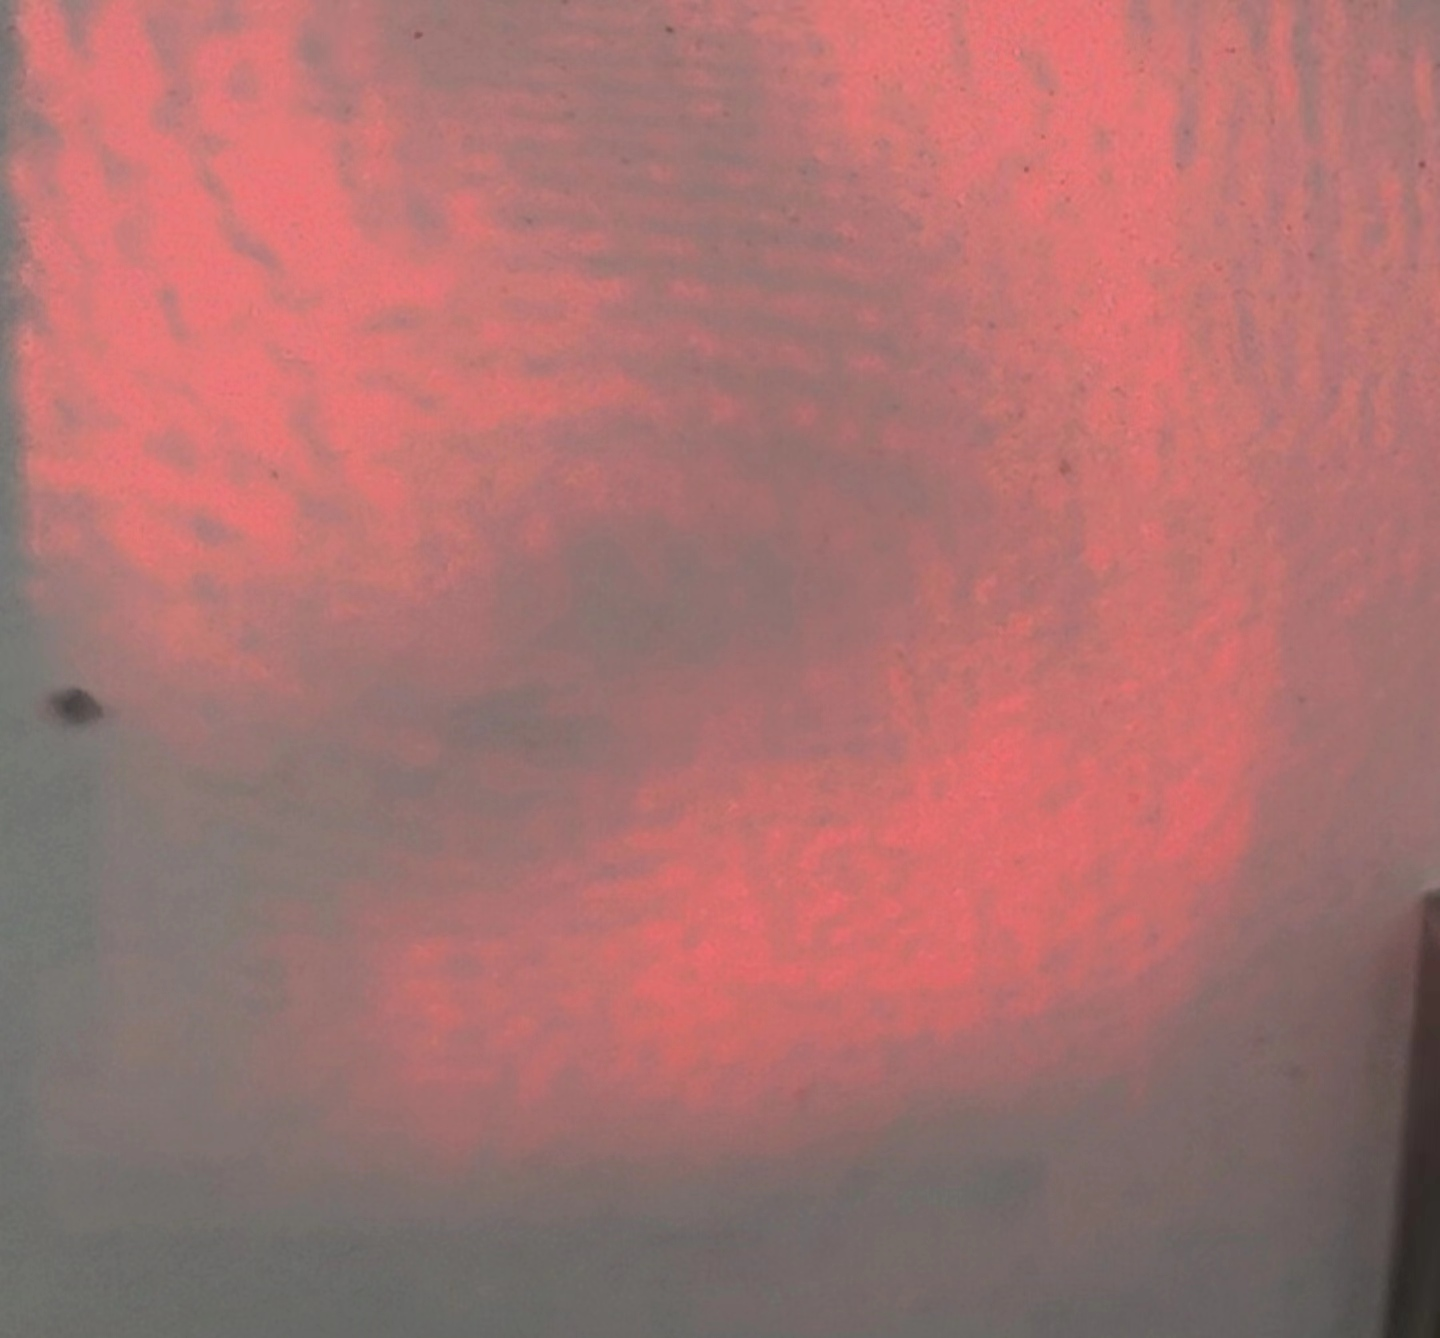
\includegraphics[width=0.4\linewidth]{images/等倾干涉}
		\caption{干涉条纹}
		\label{干涉条纹}
	\end{figure}
	注:实验效果很好,但是由于手机相机问题,可能效果不是很清晰。
		\subsubsection{测量钠双黄线的波长差}
	\begin{enumerate}
		\item 调节M1,使咸小光程差$L$,直到光程差近似为零,圆环几乎消失。
		\item 取下扩束镜,改用溴钨灯,并在灯前放置毛玻璃。将观察屏改为平面玻璃反射。
		\item 调节M2后的三颗螺钉,以及调节M1位置,观察到黄黑相间的直残状条纹。
		\item 调节精密测微头,移动反射镜M1,让条纹从模糊到清晰再到模糊。
		\item 计算钠双黄线的波长(理论值:入射波长为$589.0$nm,反射波长为$589.6$nm),并记录测量结果如下。
	\end{enumerate}
	\begin{table}[H]
		\centering
		\begin{tabular}{|c|c|c|c|}
			\hline
			实验次数 & 模糊/mm & 清晰/mm & 模糊/mm \\ \hline
			1       & 10.328  & 16.039 & 21.636 \\ \hline
			2       & 10.162  & 16.334 & 21.652 \\ \hline
		\end{tabular}
		\caption{实1验数据}
		\label{tab:data}
	\end{table}
		\begin{figure}[H]
		\centering
		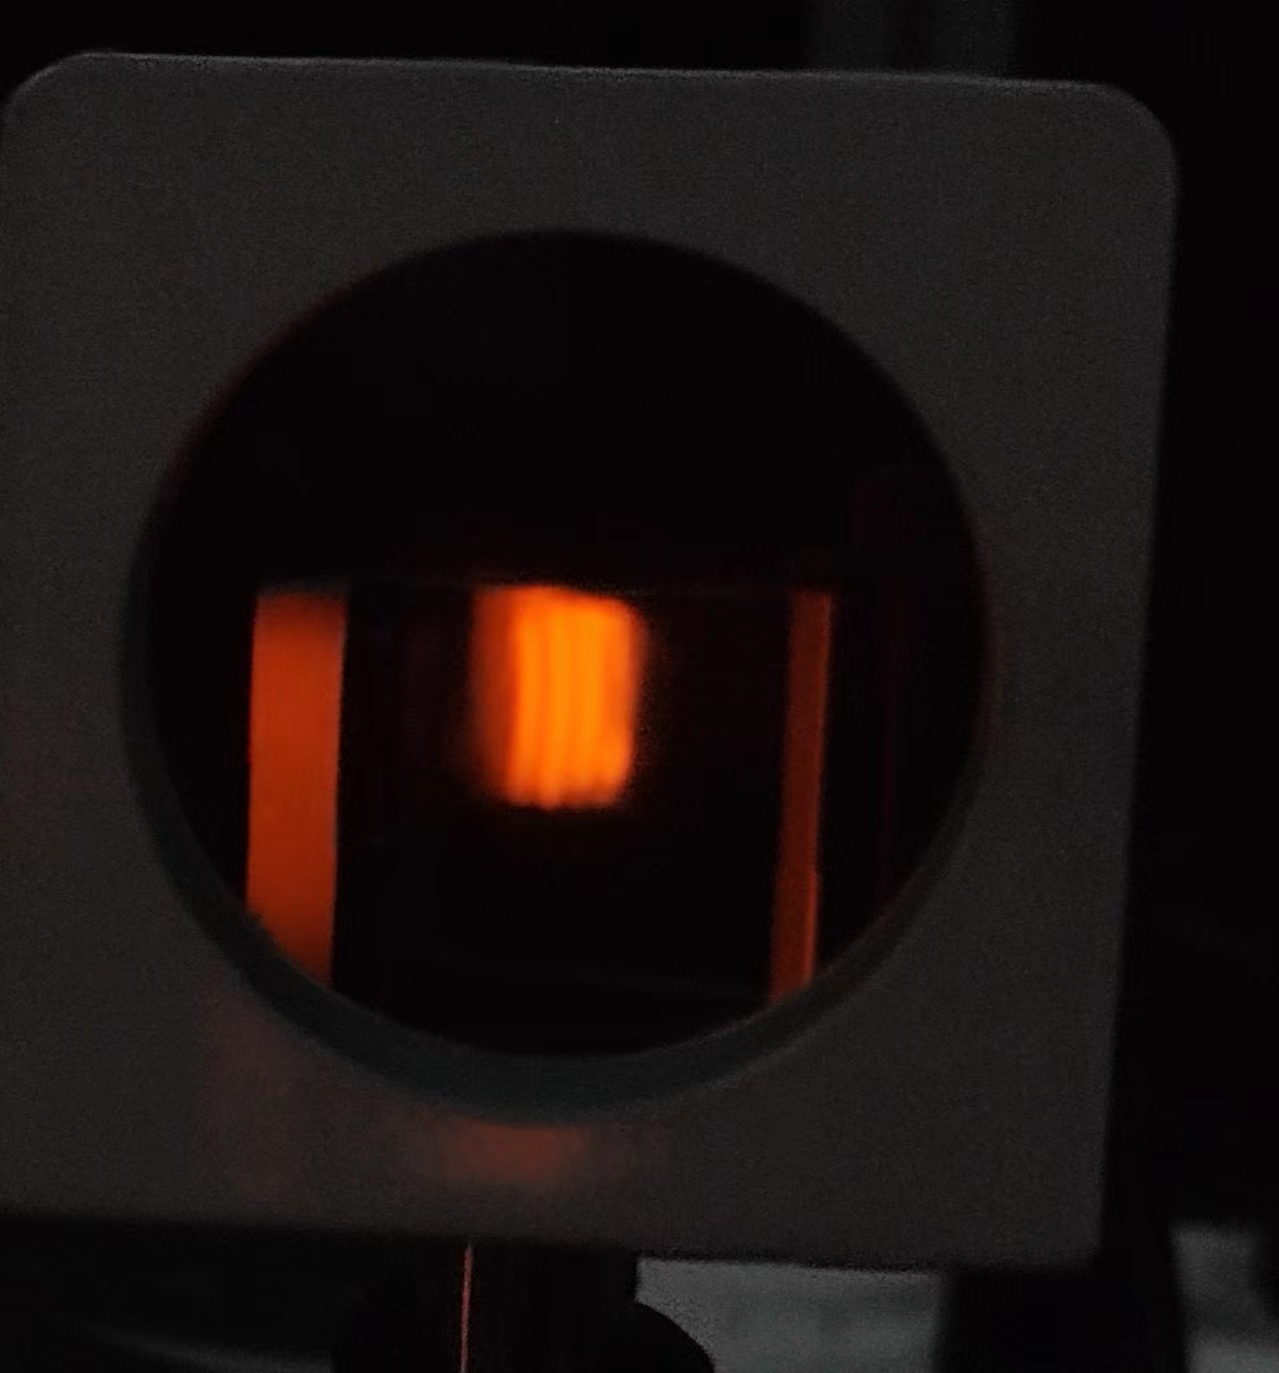
\includegraphics[width=0.4\linewidth]{images/双黄线}
		\caption{实验效果}
		\label{双黄线}
	\end{figure}
		\subsubsection{利用白光干涉测定透明薄片的厚度 t 或折射率 n }
	\begin{enumerate}
		\item 首先,调出激光干涉的等倾圆环,以减小光程差,使条纹变稀,只剩下少数几个圆环。此时,两臂光程几乎相等。
		
		\item 其次,撤掉扩束镜,换上汞灯,微调M背面的三个螺钉,观察到等倾干涉圆环。接着,调节测微头,直到屏上只剩下大圆环。然后换上白光光源(溴钨灯加毛玻璃),再次微调精密训微头,在视场中观察到彩色条纹。这些彩色条纹中间有一条全黑的暗纹,称为中心暗纹。
		\item 接下来,缓慢调节仙精密测微头,使中心暗纹移到视场中央,并记录此时读数$d1$。安装透明薄片,再次调节精密测微头,直到重新观察到彩色条纹,并将暗纹移到视野中央。记录此时精密测微头读数$d2$。
		
		\item 最后,测量薄片厚度$t$,并计算折射率$n$。实验效果如下:
		
			\begin{figure}[H]
			\centering
			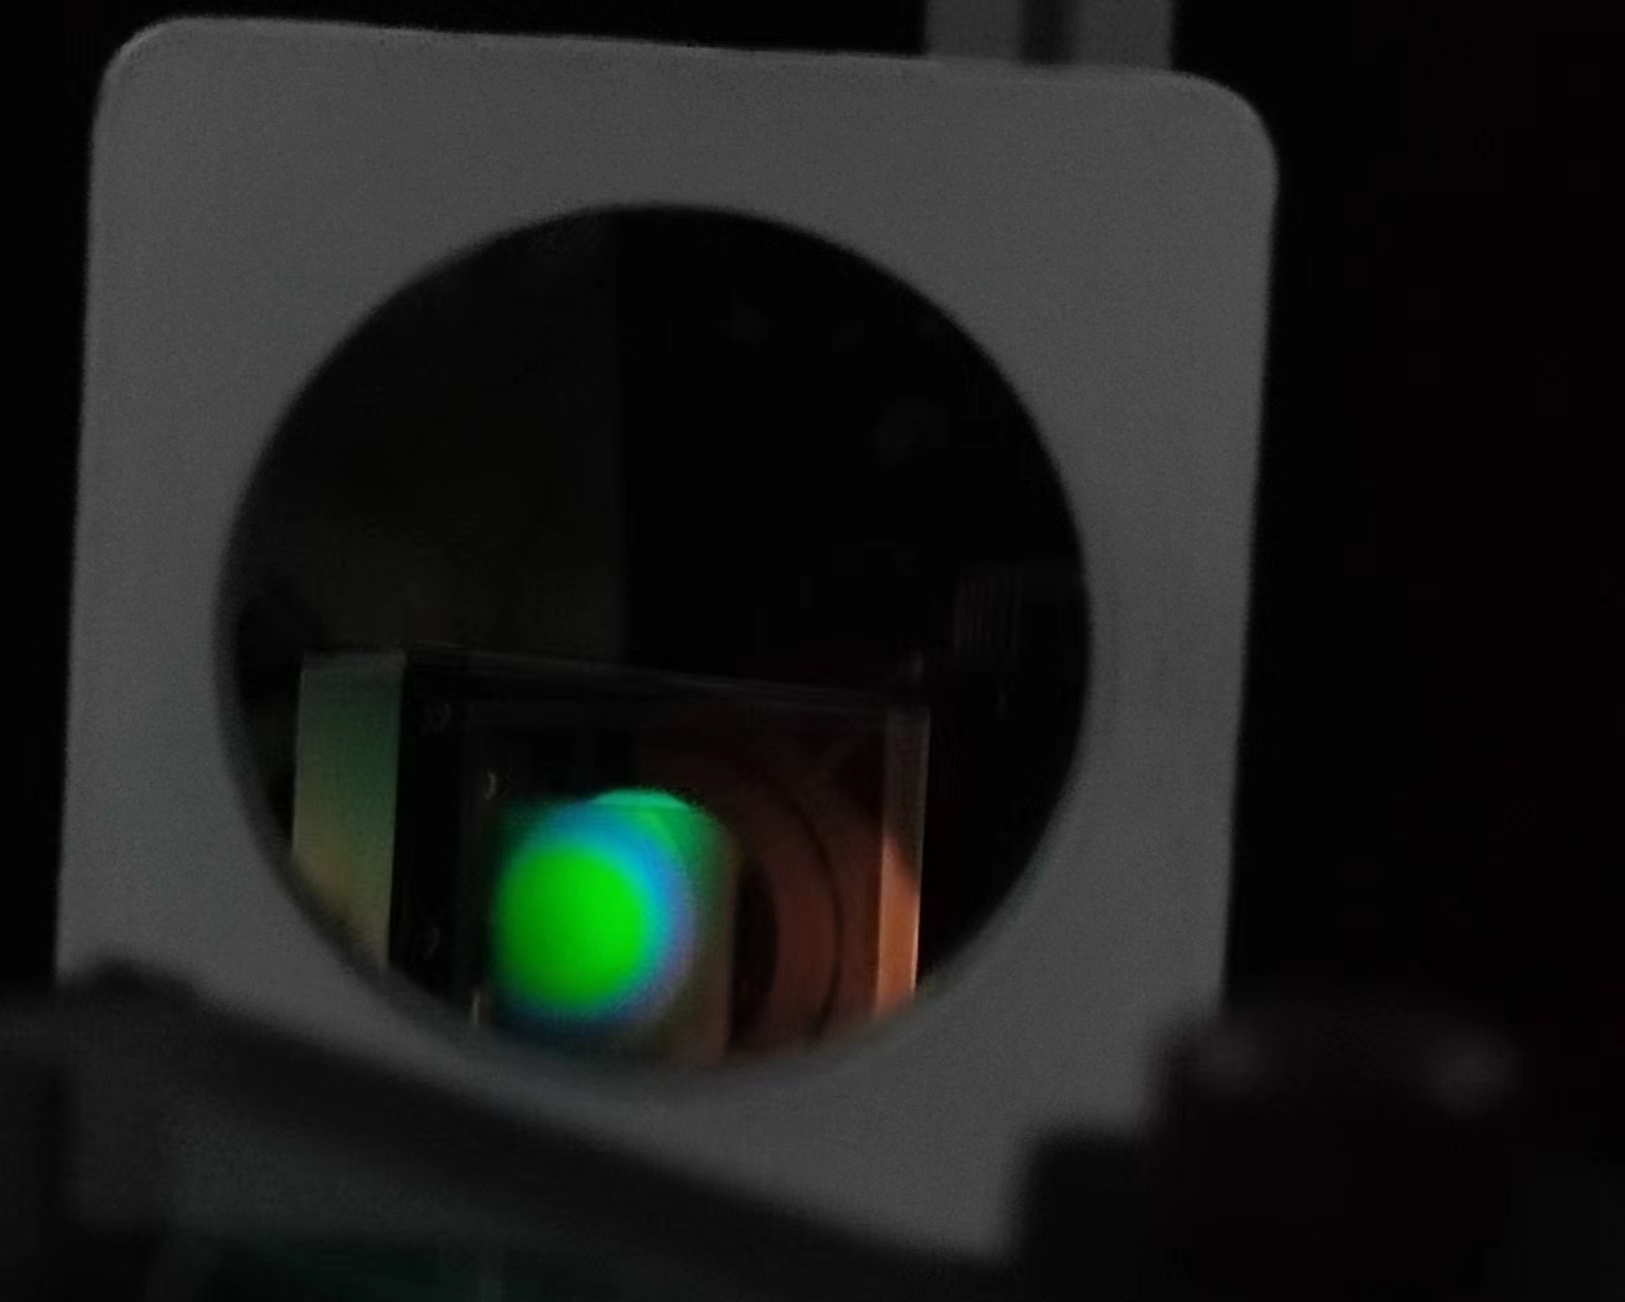
\includegraphics[width=0.3\linewidth]{images/汞灯}
			\caption{汞灯实验效果}
			\label{实验效果}
		\end{figure}
			\begin{figure}[H]
			\centering
			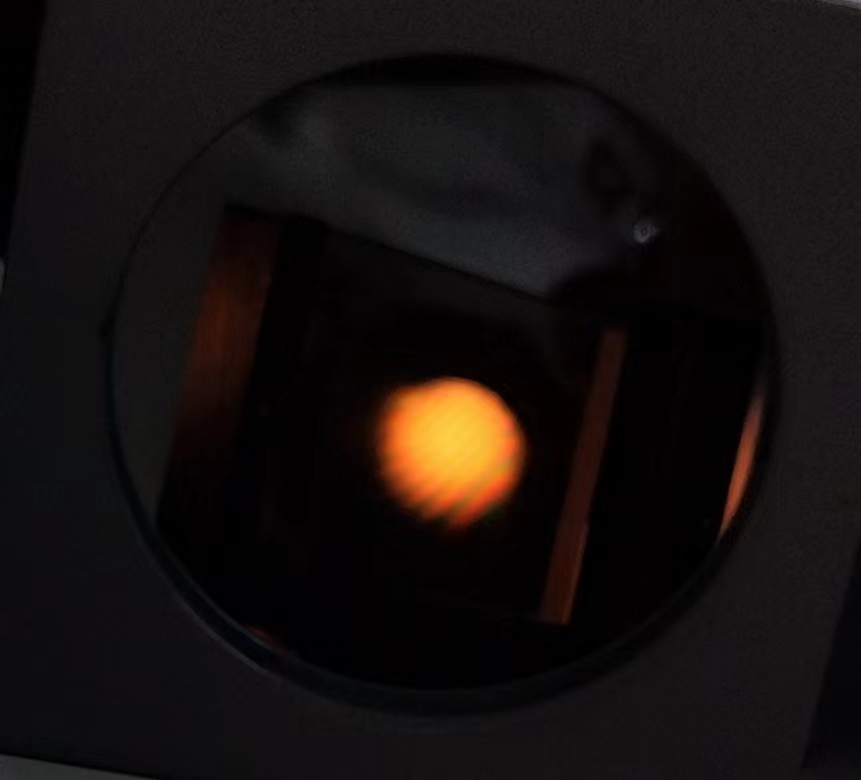
\includegraphics[width=0.3\linewidth]{images/白光}
			\caption{白光干涉实验效果}
			\label{白光}
		\end{figure}
		\begin{table}[H]
		\centering
		\begin{tabular}{|c|c|c|c|c|c|c|}
			\hline
			实验次数 & 1 & 2 & 3 \\ \hline
			$d_{1}/mm$  & 3.510 & 3.482 & 3.466  \\ \hline
			$d_{2}/mm$  & 6.724 & 6.672& 6.542  \\ \hline
			薄片厚度  & 0.163 & 0.160& 0.163  \\ \hline
			
		\end{tabular}
		\caption{实验2数据}
		\label{tab:experiment}
		\end{table}
		\end{enumerate}
	

	% 问题记录
	\subsection{实验过程遇到问题及解决办法}
	\begin{enumerate}
		\item 由于实验仪器的问题,在两位老师的帮助下也依旧没有调出干涉图像,最终选择换了一台仪器,很快就调出来了,在这里也要感谢柳老师的热心帮助,顺利完成了实验。
		\item 在钠双黄线的实验中,由于对于清晰和模糊的判定无法准确界定,可能会出现误差较大的情况,只能大致测量。
		\item 相关讨论请见后记。
	\end{enumerate}

	
	
	% 分析与讨论	
	\clearpage
	
	% 顶栏
	\begin{table}
		\renewcommand\arraystretch{1.7}
		\begin{tabularx}{\textwidth}{|X|X|X|X|}
			\hline
			专业:& 物理学 &年级:& 2022级\\
			\hline
			姓名: & 黄罗琳 & 学号:& 22344001\\
			\hline
			日期:& 2024/3/7 & 评分: &\\
			\hline
		\end{tabularx}
	\end{table}
	% ---
	
	% 小标题
	\section{迈克尔逊干涉及应用(白光干涉) \quad\heiti  分析与讨论}
	% ---
	
	% 数据处理
	\subsection{实验数据分析}

	%
	\subsubsection{测量钠双黄线的波长差}
	\begin{enumerate}
		\item 实验结果计算\\
		根据公式$\Delta\lambda=\lambda_{2}-\lambda_{1}=\frac{\lambda_{2}\lambda_{1}}{2\Delta d}=\frac{\lambda^{2}}{2\Delta d}$。\\
		根据第一次实验数据\hspace{0.2cm}
		$\Delta d_{1}=\frac{d_{2}-d_{1}}{40}=0.2827mm$\hspace{0.2cm}
	  $\Delta\lambda_{1}=\frac{\lambda^2}{2\Delta d}=0.614nm$\\
	  根据第二次实验数据\hspace{0.2cm}
		$\Delta d_{2}=\frac{d_{2}-d_{1}}{40}=0.2872mm$\hspace{0.2cm}
			$\Delta\lambda_{2}=\frac{\lambda^2}{2\Delta d}=0.604nm$\\
			最终取$\Delta\lambda=0.609nm$\hspace{0.2cm}
			相对误差$r=\frac{0.609-0.600}{0.600}=1.5\%$
			\item 误差来源分析\\
			尽管实验通过一系列操作为了使得两臂光程一致,消除光程差,但是由于人眼的局限性和设备精度的问题,很难将光程差完全消除。\\
			此外由于对于模糊清晰的判定存在严重的主观问题,此举也会引入误差。\\
			精密测微头的读数也会存在误差,在实验过程中,有时尽管旋转测微头,但是不会出现读数变化,这样也会引入误差。\\
			为找到合适的图像,需要多次进行来回反复调节,这样也会导致测微头不是只向同一个方向转动,从而引入误差。
	\end{enumerate}
	
	%
	\subsubsection{ 利用白光干涉测定透明薄片的厚度 t 或折射率 n}
	\begin{enumerate}
		\item 数据计算\\
		$\overline{t}=0.162mm$\\
			$\Delta d_{1}=\frac{d_{2}-d_{1}}{40}=0.0803mm$\hspace{0.2cm}$n_{1}=\frac{\Delta d}{t}+1=1.495$\\
			$\Delta d_{2}=\frac{d_{2}-d_{1}}{40}=0.0804mm$\hspace{0.2cm}$n_{2}=\frac{\Delta d}{t}+1=1.496$\\
			$\Delta d_{3}=\frac{d_{2}-d_{1}}{40}=0.0830mm$\hspace{0.2cm}$n_{3}=\frac{\Delta d}{t}+1=1.512$\\
			$\overline{n}=1.501$
				\item 误差来源分析\\
				根据实验测量数据得知,薄片的厚度并不均匀,存在一定的误差。
				\item 对于彩色干涉条纹的中心暗纹移至中心的界定也存在主观影响,\textbf{不过根据实验结果判断,实验相对成功}。\\
				\textbf{此外根据实验数据中d的数据显示,可能存在由于测微头多次反方向旋转引入的误差。}
				
		
	\end{enumerate}
	

	% 实验后思考题
	\subsection{实验后思考题}
	
	%思考题1
	\begin{question}
		 当空气温度变化时,空气折射率也会发生变化,请思考如何测得空气折射率?\\
		 类似于测量透明介质的实验,\textbf{实验最根本在于将透明介质放于光路中,观察前后变化},故我们可以将实验中一部分光路可以在真空与空气间相互切换,测得相关参数后,与测量透明介质的实验相同的计算方法,可以算出折射率。然而,由于空气的折射率会随着温度的变化而变化\textbf{,在实验中需要保持空气温度不变},可以将实验装置放置在恒温环境中,以有效防止温度的变化对实验结果的影响。\textbf{此外,还要检测环境的气压,防止气压变化导致折射率测量出现误差。}
	\end{question}
	\begin{question}
		对于汞灯相干长度测量问题。\\
		完成实验过程中,我发现找不到准确干涉条纹的主要原因是测微头转动,原本调整好的圆环中心会一步步偏移,从而观察条纹消失时根本无法确定是本身消失了还是我们没有观察到,在预习报告中我提到这种问题是可预见的,在实验过程中我通过将M1完全垂直于实验台面,这样会减少精密测微头调节位置时所带来的竖直方向上的光线的位移,从而使得原本的问题得到初步解决,这样相比于不这样操作,使得对于圆环中心的把控更加容易了。
	\end{question}
	
	

	
	% 小标题
	\section{迈克尔逊干涉及应用(白光干涉) \quad\heiti  后记}
	% ---
	
	% 总结、杂谈与致谢
	\subsection{实验心得体会}
	\begin{enumerate}
		\item 该实验相比于上学期迈克尔逊激光干涉实验难度剧增,主要是白光的相干长度较短,很难找到较好的实验图像。
		\item 实验仪器可能存在一些问题,导致尽管从激光,钠灯,汞灯,最后到白光干涉属于一步步精确的过程,但是随着精密测微头的转动,中心区域依旧会逐步偏离,从而导致了实验一次次失败,失之毫厘谬以千里。
		\item 实验原理方面与激光干涉相差不大,主要难度在于找到白光干涉条纹,比较考验耐心和毅力,当然标准的实验操作之后,也会很快就找到了。
		\item\textbf{ 正如我在思考题2中所提到的调整M1问题,与之配合还有另外一套实验方法,在实验过程中,我们可以在实验中将溴钨灯和汞灯放在一起,通过旋转操作可以很快的调整圆环中心位置(汞灯来检测是否跑偏),最终实验通过这种方式成功了。}
	\end{enumerate}
	% 附件

	\subsection{附件}
	\begin{figure}[H]
		\centering
		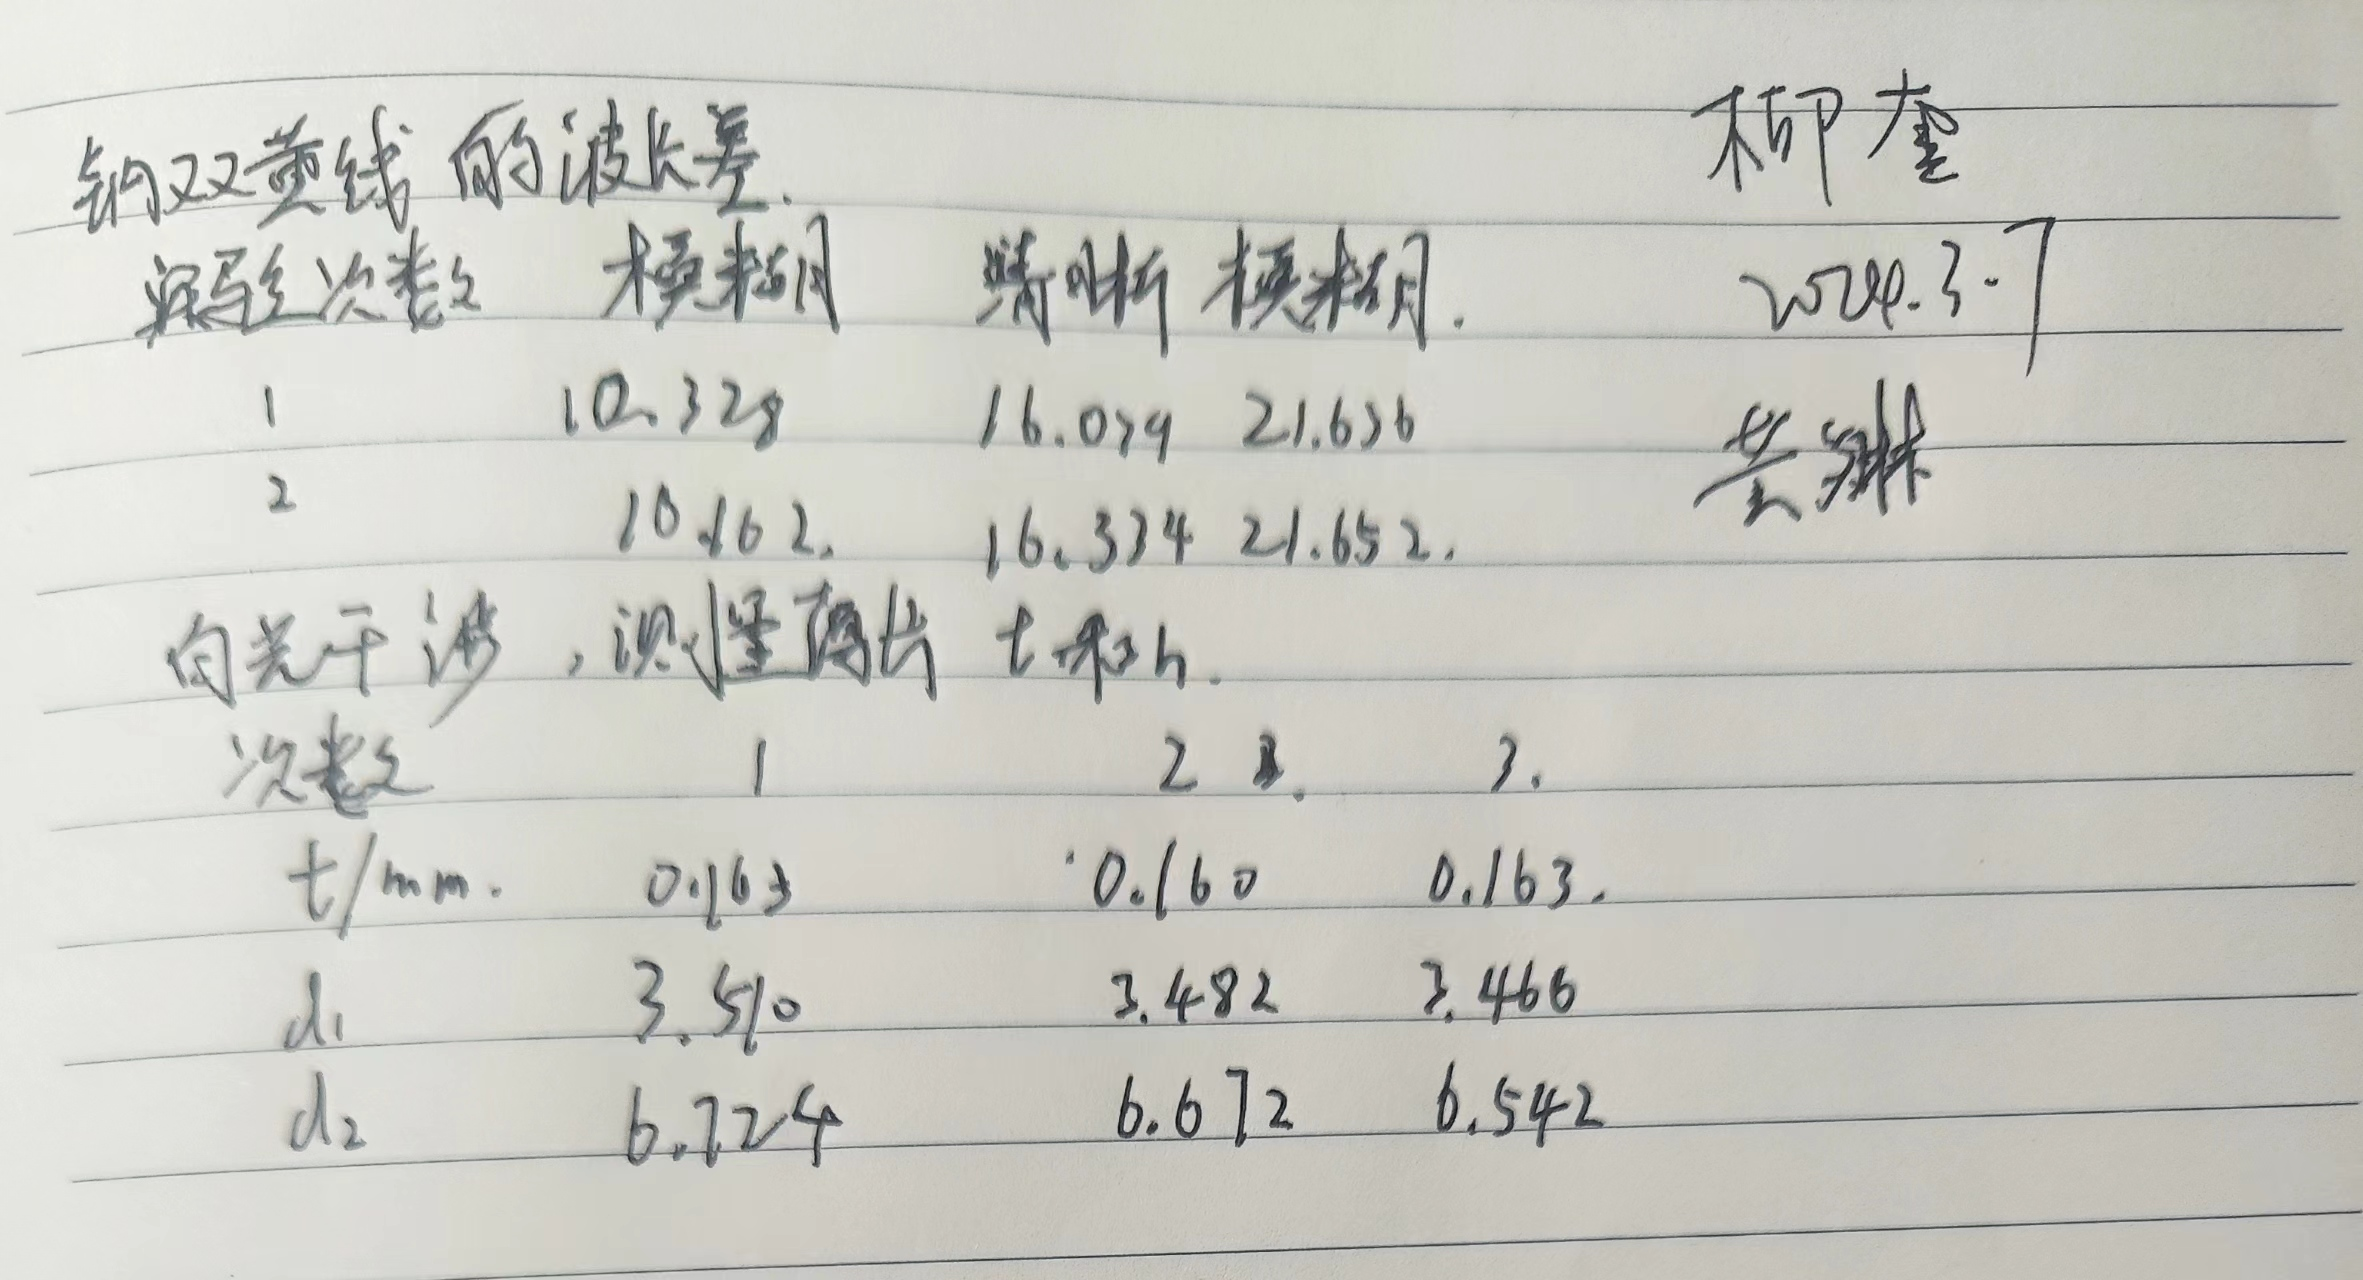
\includegraphics[width=0.2\linewidth]{images/数据}
		\caption{原始数据}
		\label{fig:}
	\end{figure}
	
	
	
\end{document}